%! Tex Root = ../proposal.tex

\begin{frame}{Personal Research}

Mention my previous research

Show how it supports and solves some of the issues mentioned in the challenges

Quick summary of previous research
\end{frame}

% Intro to the reachability idea
\begin{frame} %-----------------------------%
\frametitle{Reachability Set}
  \begin{itemize}
  \item Reachable set on Poincar\'e section
        \begin{itemize}
            \item The set of states that can be attained from a given initial state via admissable control input
            \item Enlarge the intersection region on the Poincar\'e section
        \end{itemize}
  \item \emph{Computational Geometric Optimal Control}
    \begin{itemize}
        \item Poincar\'e section defined by \( \alpha_d \) in \( m_1\)
        \item Direction on Poincar\'e section defined by \( \theta_d \) in \( m_2 \)
    \end{itemize}
 \end{itemize}
  \begin{align*}
    J &= -\frac{1}{2} \left( \bar{x}(N) - \bar{x}_{n}(N)\right)^T Q_f\left( \bar{x}(N) - \bar{x}_{n}(N)\right)\\
    m_1 &= 0 = \frac{y(N) - L_{1y}}{x(N) - L_{1x}} - \tan{\alpha_d} \\ 
    m_2&= 0 = \frac{\dot{x}(N) - \dot{x_n}(N) }{x(N) -x_n(N) } - \tan{\theta_d} \\
     0 &\geq\bar{u}^T \bar{u} - u_{max}^2 
    \end{align*}

    \note[itemize]{
        \item E-L equations are used to derive necessary conditions for optimality
        \item Results in TPBVP and indirect optimal control
        
    }
\end{frame}   %-----------------------------%

% benefits of variational integrator

% results from 2015 AAS
\subsection*{Circular Restricted Three Body Problem}
\begin{frame}[t]\frametitle{CRTBP}
    Motion about CRTBP

    Implemented variational integrator

    Demonstrated use of \Poincare section and reachability



\end{frame}

\begin{frame}%--------------------------------------------%
\frametitle{Transfer Problem}
    \begin{itemize}
        \item Transfer from \( L_1 \) orbit to periodic orbits near the Moon
        \item Bounded control input and fixed time horizon
    \end{itemize}
    \begin{figure}
        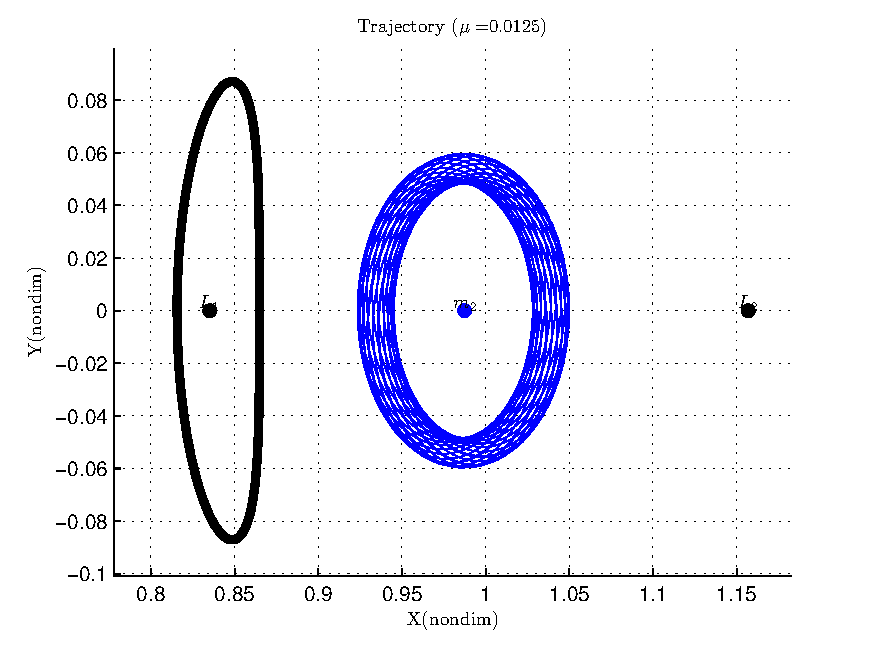
\includegraphics[width=0.7\textwidth]{moon_orbit}
    \end{figure}
    
    \note[itemize]{
        \item Introduce problem
        \item Possible use as a communication array
        \item Might actually be a distant retrograde orbit
        }
\end{frame} %--------------------------------------------%

\begin{frame}%------------------------------------------------%
\frametitle{Reachable Set Transfer}
\begin{itemize}
    \item Reachablility set generated on Poincar\'e section
    \item<3-> Intersection point used to generate a transfer
\end{itemize}
    \begin{figure} 
    \centering 
    \begin{subfigure}[htbp]{0.5\textwidth} 
        \only<1-2>{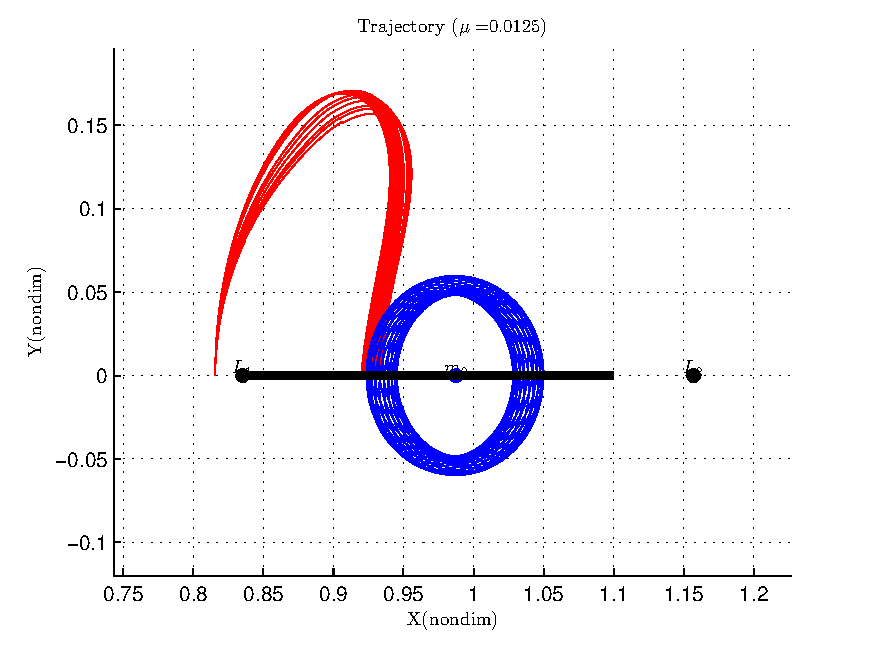
\includegraphics[width=\textwidth]{reach_trajectory}  }
        \visible<3->{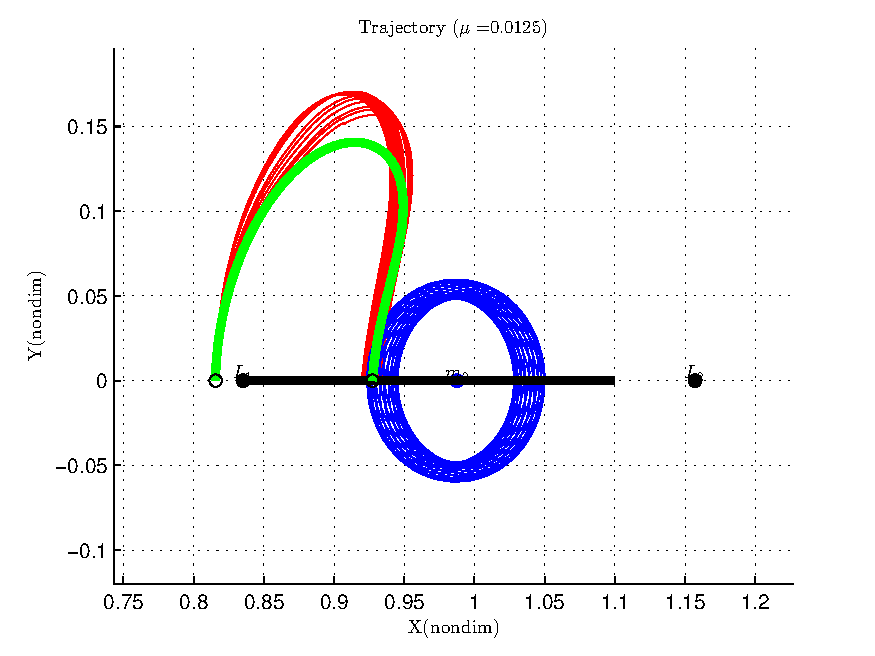
\includegraphics[width=\textwidth]{reach_transfer}  }
    \end{subfigure}~
    \begin{subfigure}[htbp]{0.5\textwidth} 
        \visible<2->{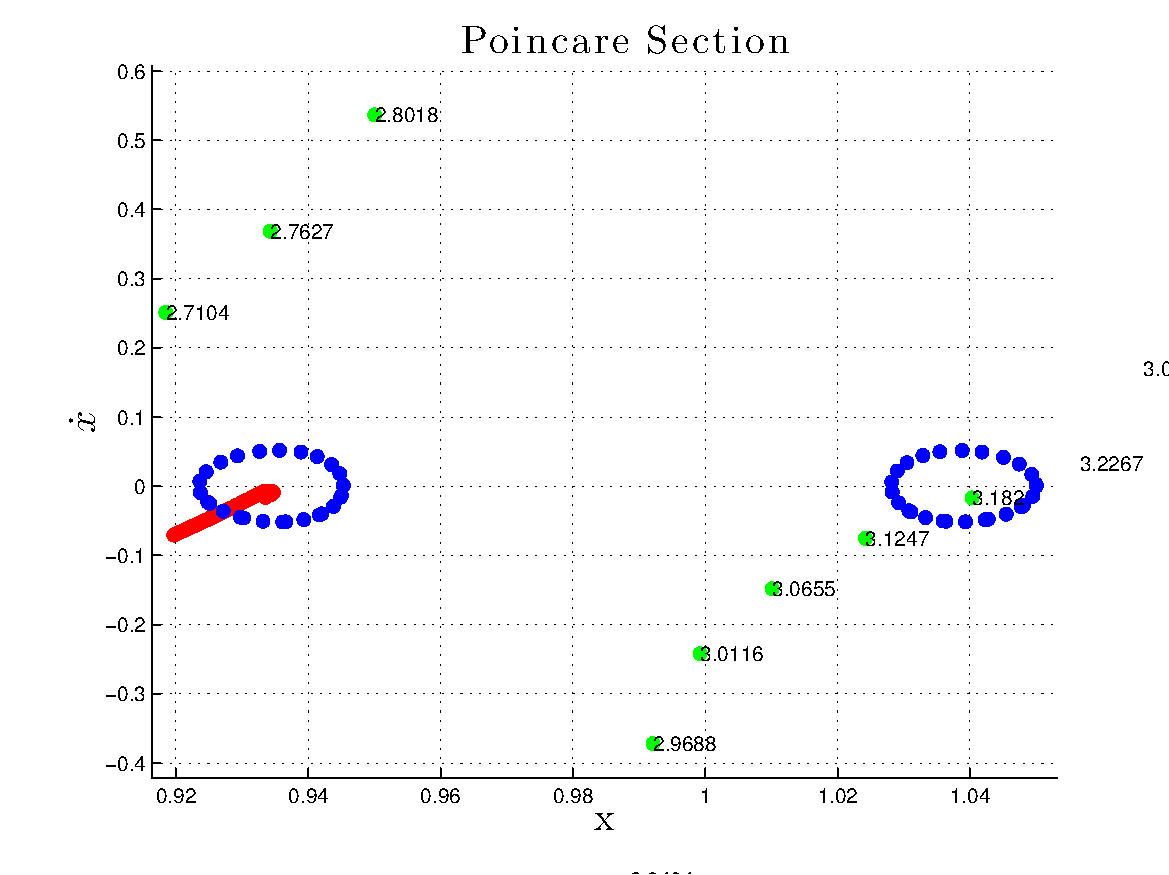
\includegraphics[width=\textwidth]{poincare_compare} }
    \end{subfigure} 
    \end{figure}
    
        \visible<4->{
    \begin{itemize}
        \item  Reachable set intersect the target 
        \item Shorter time of flight \( t_f \approx 1.4 \)
    \end{itemize}
    }
    \note[itemize]{
        \item Compare to reachable set approach
        \item Shorter time of flight
        \item Multiple shooting to solve TPBVP
        Vary \( \theta\) to change direction on section
        Linear interpolation to determine intersection on Poincar\'e section
        }
\end{frame} %--------------------------------------------------%

% Differences when considering an asteroid - polyhedron model

% Results from 2016 AAS



\begin{frame}[t]\frametitle{Asteroid Paper}
    
Extended reachability and \Poincare to more challenging enviornment 

Gravity model is much more complex and dynamics are highly perturbed

\end{frame}

% Results from 2016 ACC

\begin{frame}[t]\frametitle{Constrained Attitude Control}
    
geometrically exact representation of system configuration allows for global stability

Attitude control in the presence of constraints

\end{frame}